\documentclass[conference]{IEEEtran}

\IEEEoverridecommandlockouts

\usepackage{amsmath}
\usepackage{graphicx}
\usepackage{array}
\usepackage{eso-pic}

\newcommand\AtPageUpperMyleft[1]{\AtPageUpperLeft{
\put(\LenToUnit{0.014\paperwidth},\LenToUnit{-1cm}){
  \parbox{0.5\textwidth}{\raggedleft\fontsize{8}{11}\selectfont #1}}
}}

\newcommand{\conf}[1]{
\AddToShipoutPictureBG*{
\AtPageUpperMyleft{#1}
}}

\def\BibTeX{{\rm B\kern-.05em{\sc i\kern-.025em b}\kern-.08em
    T\kern-.1667em\lower.7ex\hbox{E}\kern-.125em}}

\makeatletter

\newcommand{\linebreakand}{
  \end{@IEEEauthorhalign}
  \hfill\mbox{}\par
  \mbox{}\hfill\begin{@IEEEauthorhalign}
}

\makeatother

\begin{document}

\raggedbottom

\conf{2021 international conference on ICT for emerging regions (ICTer)}

\title{English Language Trainer for Non-Native Speakers using Audio Signal Processing, Reinforcement Learning, and Deep Learning}

\author{
\IEEEauthorblockN{
\textit{
H.C.R. Jeewantha, A.N. Gajasinghe, N.I. Naidabadu, T.N. Rajapaksha, D. Kasthurirathna, A. Karunasena
}}
\IEEEauthorblockA{
\textit{
Faculty of Computing, Sri Lanka Institute of Information Technology,
} \\
Malabe, Sri Lanka
\\
\textit{
\{it18151220, it18153682, it18148350, it18149654\}@my.sliit.lk, \{dharshana.k, anuradha.k\}@sliit.lk
}}
\and
}

\maketitle

\begin{abstract}
Lack of basic proficiency and confidence in writing and speaking in English is one of the major social problems faced by most non-native English speakers. Although the general adult literacy rate in Sri Lanka is above average by world standards, the English literacy rate is just 22\% among the Sri Lankan adult population. Many individuals face setbacks in achieving their career and academic goals due to these language barriers. In a world where English has become a compulsory requirement to pursue higher education, career development, and performing day-to-day activities, ``English Buddy'' is a software solution developed to enhance the English learning experience of individuals in a more personalized and innovative way. The system provides an all-in-one solution while filling major research and market gaps in existing solutions in the e-learning domain. The system consists of a personalized learning environment, automated pronunciation error detection system, automated essay evaluation process, automated descriptive answer evaluation component based on semantic similarity, and real-time course content rating system. English Buddy is implemented using state-of-the-art technologies such as Audio Signal Processing, Reinforcement Learning, Deep Learning, and NLP. The LSTM, Sentiment Analysis, and Siamese network models have gained accuracy scores of 0.93, 0.92, and 0.81 respectively. Further, the UAT results proved that the personalized recommendations and pronunciation error detection processes are accurate and reliable. This research has been able to overcome the limitations of most existing solutions that follow traditional approaches and provide better results compared to the recent studies in the e-learning research domain.
\end{abstract}

\begin{IEEEkeywords}
Audio Signal Processing, Deep Learning, Natural Language Processing, Reinforcement Learning
\end{IEEEkeywords}

\section{Introduction}

The English language is the most common language used around the globe today [1]. It has become the international language for communication, business, and even entertainment. Therefore, English language skills have become a compulsory requirement in many fields [1, 2] like academia [3], career development, and international migration.

Globally recognized English exams like IELTS and TOEFL [3] are used as metrics of English proficiency. Most non-native English speakers around the globe including Sri Lankans struggle in these English exams. Hence, they suffer setbacks in achieving their career and academic goals and miss out on valuable opportunities.

Specially, Sri Lankan students who study English as a secondary language in schools struggle to obtain reasonable grades even in local exams like GCE Ordinary Level and Advanced Level exams. Although Sri Lanka's overall adult literacy rate is significantly greater than the world and regional norms which is almost 92\% in the year 2018 [4], the English literacy among Sri Lankans over 15 years of age is only 22\% [5]. Hence, English a major concern most Sri Lankans face daily in their day-to-day life.

With the advancement of ICT, most people have become familiar with e-learning platforms and have experienced their benefits such as learning at their own pace at their preferred time [6]. At present, especially, due to the current situation of not only in Sri Lanka but the whole world with the Covid-19 pandemic, the value of e-learning has risen massively due to social distancing guidelines. Most of the schools and universities [8] have started offering lessons and exams online adhering to the social distancing guidelines by governments to limit the spread of the pandemic [8].

This paper presents a smart interactive software platform called ``English Buddy'' consisting of writing and speaking activities that students are tested on, in any locally or globally recognized English exam. The student answers are automatically evaluated by the system and feedback is provided. The system also consists of a recommendation system that suggests learning material to the students based on their recognized weaknesses and previous performances.

The application is implemented using cutting-edge technologies such as Audio Signal Processing, Reinforcement Learning, Deep Learning, NLP, and Sentiment Analysis to create an innovative platform for non-native English speakers to overcome the above-mentioned problems.

Reinforcement Learning is a branch of machine learning that studies how intelligent agents can behave in a given environment to maximize the concept of cumulative reward [7]. NLP is a field of AI that gives computers the ability to read, understand and derive meaning from human languages [10]. Sentiment analysis analyzes if the underlying sentiment of a text is positive, negative, or neutral. Audio Signal Processing is the study of speech signals and the processing techniques of those signals [12]. Deep Learning is a subset of machine learning that deals with algorithms that are motivated by the structure and the function of the human brain [19].

The rest of the paper is organized as follows: Section II presents a background of prior similar research, section III describes the methodology, section IV presents the results, and the limitations and future work are discussed in section V.

\section{Background}

Since English has become the most widely used language in the world, most people are involved in learning English daily as beginners [1, 2, 3]. With the increasing demand, more research has been conducted on learning the English language in the e-learning domain recently [9, 10] with little success.

With the advancement of computing and multimedia, there has been a new interest in Computer-Assisted Pronunciation Teaching (CAPT) applications in recent years. Pronunciation errors could be classified into 2 main types called phonemic and prosodic errors. By extracting the features of those errors, much research has measured the pronunciation level of a speaker in different ways. The likelihood-based scoring feature initially used in the 1990s, saw the creation of several likelihood-based phoneme-level error detection algorithms. For example, Kim, Franco, and Neumeyer [11] used log-likelihood scores in forced alignment mode. Expanded versions of likelihood-based scores were successfully used by Mak et al [12]. Prosodic pronunciation error detection is a very detailed discussion in CAPT systems [13]. Bernstein, Cheng, and Suzuki [14] have shown that there is a linear relationship between fluency measures and human judgments of proficiency. Mueller, Wet, Walt, and Niesler [15] applied phoneme-level log-likelihood scoring to speech from near-native language learners. However, the Goodness of Pronunciation (GOP) score did not correlate with human ratings [15].

Although the e-learning industry has grown rapidly in the past few years, it is mainly focused on the content delivered to students. Further, the same content is delivered to every user, whereas users are different from each other in terms of their strengths and weaknesses. Much research addresses this one-size-fits-all issue. For example, Schiaffino, Garcia, and Amandi [16] proposed an intelligent agent-eTeacher by victimization Bayesian network which provides personalized assistance by observing the behaviour while the student is taking online courses and automatically building the student’s profile. Halawa, Hamed, and Shehab proposed a personalized e-learning recommendation model based on the psychological type and learning style model [17] focused on student personality types and the dominant preferences based on the Myers-Briggs Type Indicator (MBTI) theory. Yanni and Ping [18], the authors of a study on personality learning in e-learning systems have implemented a recommendation engine based on trust value. The intelligent recommendation engine with user interest would help to introduce customized user attraction with the method, according to the above-mentioned values. However, only a few research focuses on user flaws and feedback to incorporate a customized course content recommendation engine.

Automated essay evaluation is a trending topic at present research. The beginning of automated essay evaluation was found in the works of Page in the 1960s [19]. In 1966, Page has proposed Project Essay Grader (PEG) which identifies a group of text features and proxies, that are considered approximations of the intrinsic variables of writing quality. However, it is only relying on linguistic features where neither NLP nor lexical content is considered [20]. Intelligent Essay Assessor (IEA) has been developed in the late 1990s, for automated essay evaluation, using Latent Semantic Analysis (LSA) [22]. Further, Mahana, Johns, and Apte suggested a solution for automated essay grading with linear regression techniques which evaluated the essays based on different parameters such as dexterity, diction, vocabulary, structure, and organization [23]. Even though there are several pieces of research done on automated essay grading, they consist of many limitations like lower accuracy, dismissing grammatical and spelling mistakes, and lack of proper feedback.

The semantic textual similarity is a heavily discussed topic in computational linguistics due to the advancements of AI-based technologies and their heavy usage in multiple domains [24] including the automatic answer evaluation. The difficulty of measuring up how much the contextual meaning of a text is reflected in another text is proven in much previous research [24]. A similar study has been conducted in an intelligent assistant for IELTS exam candidates [25] where sentence similarity was measured using cosine proximity and the Doc2Vec model. The limitation of this system is its low accuracy of 67\% [25]. Many traditional NLP-based approaches [25] with BLEU [26], n-grams [27], and algorithms for keyword matching [28] have many shortcomings such as lower accuracy due to measuring syntactic similarity instead of semantic similarity [24] as they measure the number of matching keywords present in each text. Due to the high complexities of linguistics in the English language in general, it is not possible to claim the 2 texts are similar in meaning just by matching keywords, without trying to understand the overall meaning and semantics of the text [24]. But methodologies using deep learning try to compare 2 texts based on their overall meaning [24] and provide a more reliable and accurate similarity evaluation.

\section{Methodology}

The high-level system overview diagram of the proposed system consisting of 4 major components with novel features English Buddy is shown in Fig. 1.

\begin{figure}[htbp]
\centerline{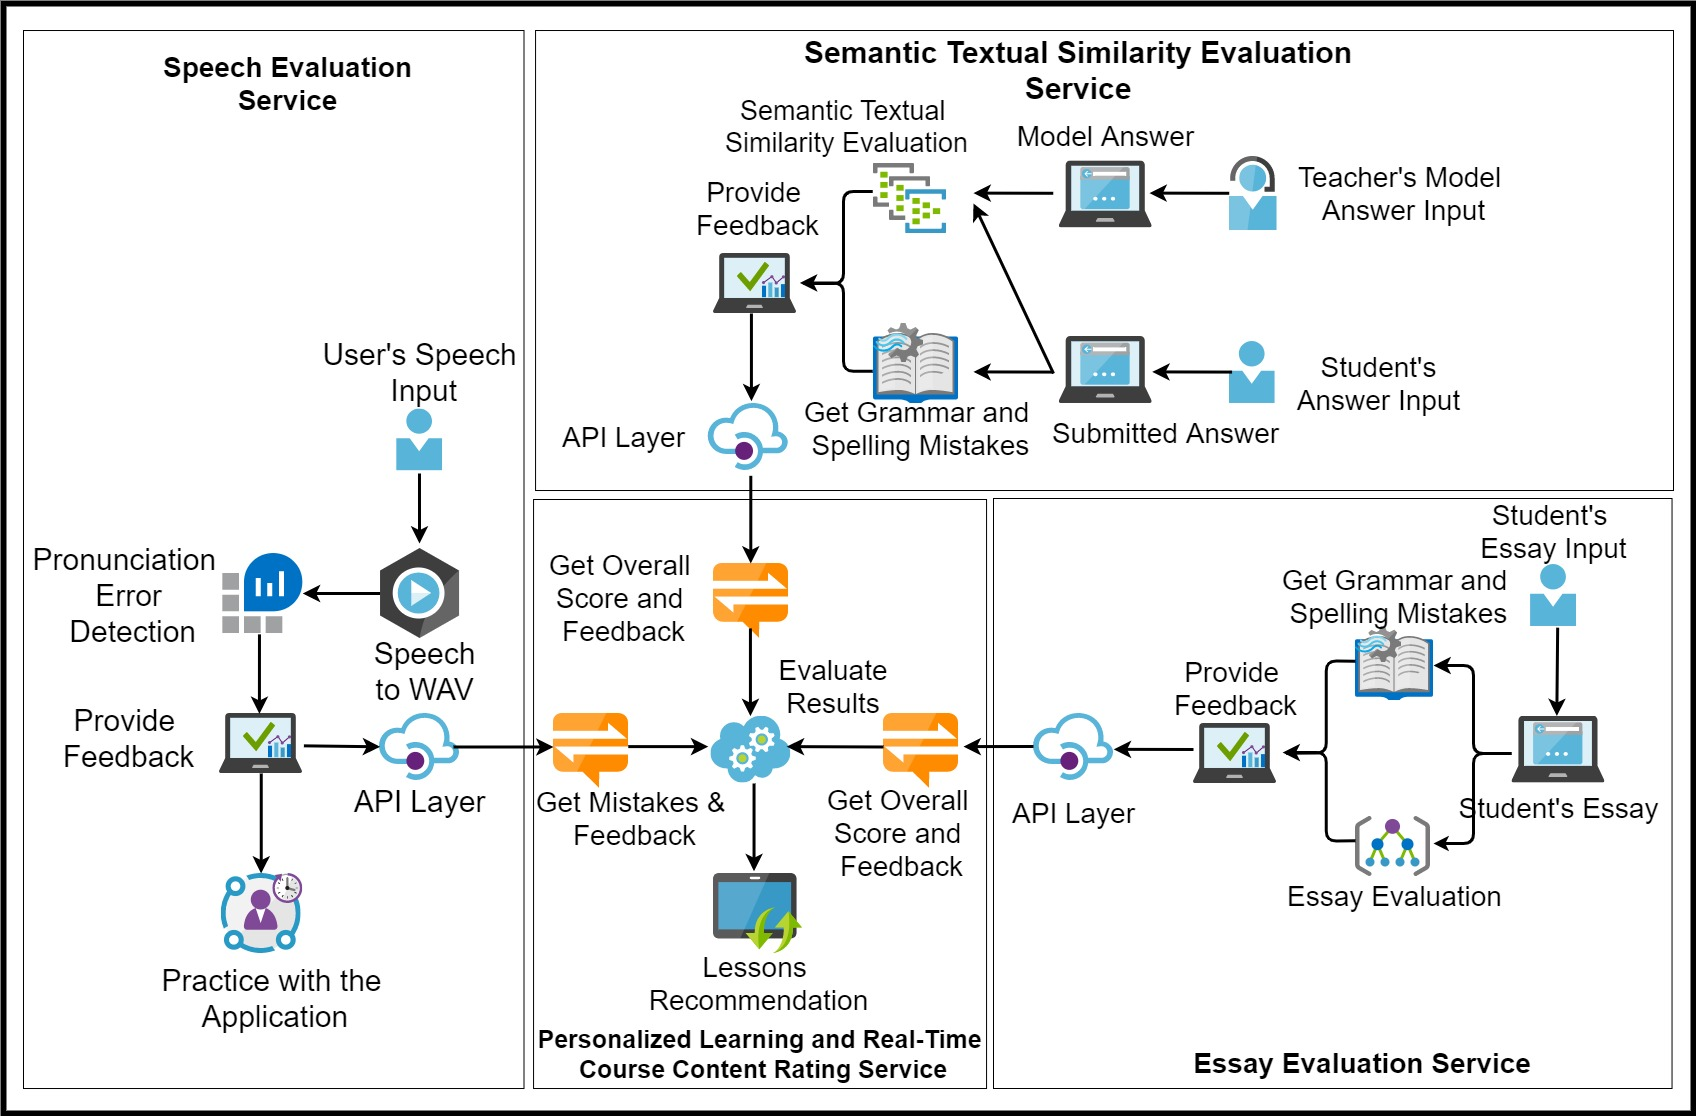
\includegraphics[scale=0.15]{team_system_diagram.jpg}}
\caption{High Level System Overview Diagram}
\end{figure}

\subsection{Automated Pronunciation Error Detection and Evaluation}

This module performs the speech analysis to identify the pronunciation level and errors. A personalized vowel chart is created to identify mispronounced words and vowels to provide the GOP value. Further, based on the pronunciation mistakes of the user, a virtual trainer teaches the user how speech could be improved.

A phoneme or speech sound is the smallest part of spoken language that makes a difference in meaning. By tracking phonemes, the system can measure the pronunciation level. Gender, age, and the native language of the speaker can affect the pronunciation. Praat tool was used to check the accuracy of the system. In the audio pre-processing stage, an open-source speech recognition toolkit named VOSK was used for speech recognition \& word segmentation as shown in Fig. 2.

\begin{figure}[htbp]
\centerline{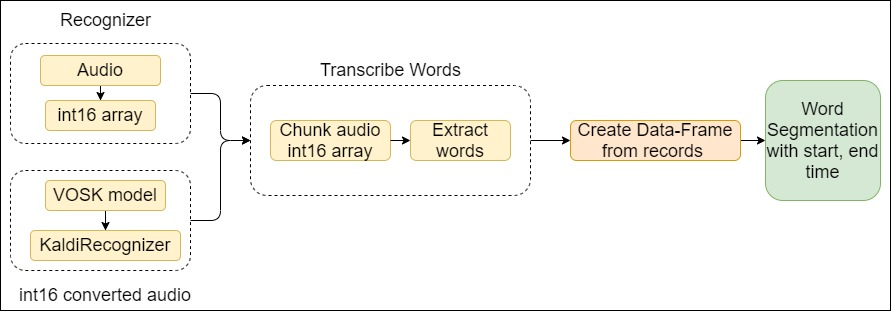
\includegraphics[scale=0.28]{it18151220_word_segemntation.jpg}}
\caption{Word Segmentation using VOSK KaldiRecognizer}
\end{figure}

Once preprocessing is done, the next step is to measure format frequency using the formant position formula. In speech science and phonetics, a formant is the broad spectral maximum that results from an acoustic resonance of the human vocal tract. The first 2 formants (f1 \& f2) are important in determining the quality of vowels and are frequently said to correspond to the open/close and front/back dimensions.

To extract the f1 \& f2 from audio, the 1st step must be the point processing throughout the audio. A point process object represents a point process, which is a sequence of points t\textsubscript{i} in time, defined on a domain (t\textsubscript{min}, t\textsubscript{max}). The index i runs from 1 to the number of points. The points are sorted by time, i.e., t\textsubscript{i} + 1 \textgreater \! t\textsubscript{i}. The point process helps to identify the voiced intervals (or glottal pulses) of the given audio file.

To detect f1 \& f2 formants within the voiced intervals, the filtered voiced intervals from the point process are re-sampled to a sampling frequency of twice the value of the formant ceiling. Then formants frequencies are measured using LPC coefficients with the algorithm using the Burg method. Then it gives f1 \& f2 formants frequencies within the voiced intervals of the given audio file. 

Vowels and consonants are the 2 main classes of speech sounds. Creating a personalized vowel chart shown in Fig. 3. can help to avoid the accent, gender, and age. f1 of monophthongal vowel sound against f2 were used to create the vowel chart as shown in Fig. 3.

\begin{figure}[htbp]
\centerline{\frame{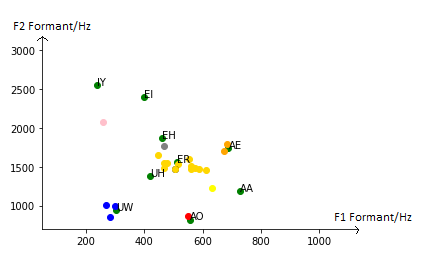
\includegraphics[scale=0.57]{it18151220_vowel_detection.png}}}
\caption{Word “Kangaroo” - Three Syllables Word - UW, ER, AE}
\end{figure}

After the above process, the system marks the top boundary and bottom boundary for all vowel formant frequency differences. By using the text transcription of the pronounced word, the system identifies the vowel pattern and specific vowels that are related to the word as shown in Fig. 4.

\begin{figure}[htbp]
\centerline{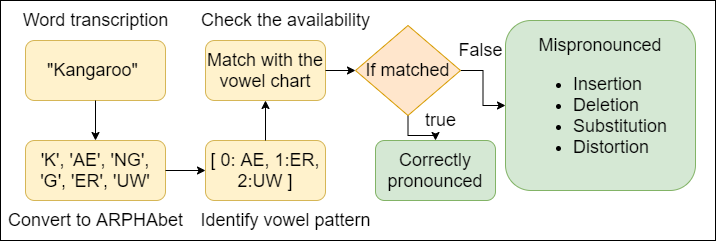
\includegraphics[scale=0.28]{it18151220_vowel_detection_flow.png}}
\caption{Vowel Detection Flow}
\end{figure}

The following types of errors can be used to measure the pronunciation level of a word.

\begin{itemize}
\item Deletion: Vowel in a word is removed while pronouncing
\item Insertion: Extra vowel is inserted while pronouncing
\item Distortion: Vowel is pronounced in a distorted way
\item Substitution: Vowel is replaced with another one
\end{itemize}

The system shows the mispronounced vowels and teaches the user how to pronounce the word correctly by using an error database. Text to speech API and lip-syncing animations were used to improve human-computer interaction in the teaching process. The system tracks all mistakes and suggests rhyming words if the user is doing the same mistake repetitively.

\subsection{Personalized Learning and Real-Time Sentiment Analysis}

The main aim of this module is to create a new customized e-learning model based on the user's weaknesses, as well as a lesson rating system based on user feedback. To achieve the above objective, when assessing a user's response for a learning activity, several criteria are considered, including relevance to the model answer, spelling and grammatical errors. According to the score obtained by the user, the agent change status and recommends course material, activities, and assignments to each user. Further, users can comment on the recommended course contents, and it is ranked according to the users’ comments. Therefore, course content providers can improve the content according to the feedback given. Fig. 5. shows the system diagram of this component.

\begin{figure}[htbp]
\centerline{\frame{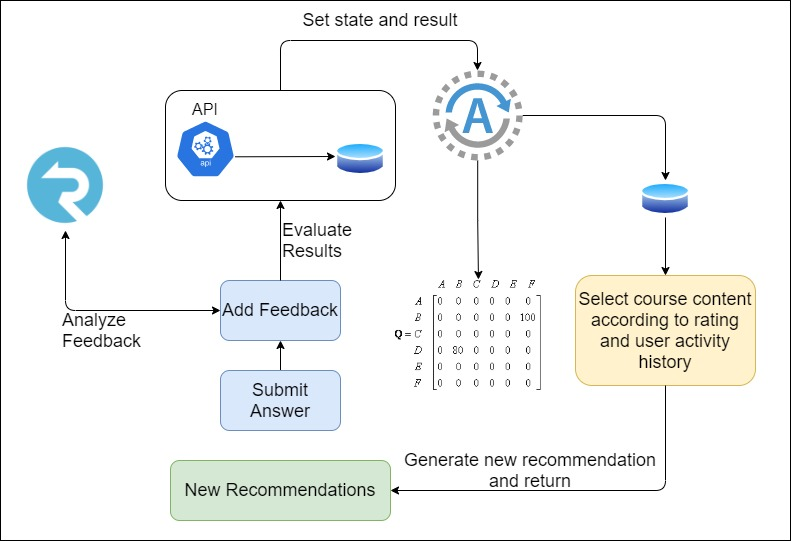
\includegraphics[scale=0.24]{it18153682_sod.jpg}}}
\caption{System Diagram for Personalized Learning System}
\end{figure}

Reinforcement learning was used for recommending lessons according to the user’s weaknesses. Since several reinforcement learning algorithms for this purpose use dynamic programming techniques, the environment is usually expressed as a Markov decision process. Q-Leaning [7], which is a model-free, off-policy algorithm, was used to find suitable courses as per the current state of the course and the user’s weaknesses.

Sentiment analysis was used to detect user comments, detect whether it is positive, negative, or neutral and rank the courses according to the results. Textual data is often subjected to sentiment analysis to assist in the monitoring of user input and to better understand user needs. Multi-class Classification sentiment analysis is done using ML.NET.

\subsection{Automated Essay Evaluation}

The automated essay evaluation functionality is based on Recurrent Neural Networks (RNN). The RNN model used in this module learns the relationships of essays and then predicts the scores for the given essay.

Kaggle Automated Student Assessment Prize (ASAP) essay data set was used for training purposes. Some initial preprocessing tasks were required before feeding the data set to the model. The NLTK library was used to do the word tokenization processes. Afterwards, the Word2Vec algorithm has used to convert word tokens into feature vectors which are required to feed to the model. Keras and TensorFlow libraries have been used to perform different deep learning tasks including feature extraction and model creation. The implemented RNN was a Long Short-Term Memory (LSTM) model which is a special kind of RNN that is capable of learning long-term dependencies in data.

The LSTM model consists of 2 LSTM layers, a dropout layer, and a dense layer. K-fold cross-validation has been used on the training phase with 5 folds. The average Cohens Kappa value, which is a statistic that measures inter-annotator agreement, is calculated by considering the Cohens Kappa value for each fold.

\subsection{Semantic Textual Similarity Evaluation}

This component focuses on evaluating the relevancy of the student's short descriptive answer by comparing its semantic textual similarity to the provided model answer using a deep learning model with Siamese network architecture [21]. Student answer is automatically evaluated based on several criteria such as relevancy to the model answer, spelling and grammar, and subjectivity of the used language style. Activities such as text summarizations and picture descriptions are used as activities students provide short descriptive answers to. The four data sets used were Quora Question Pairs (QQP), Sentences Involving Compositional Knowledge (SICK), Paraphrase Adversaries from Word Scrambling (PAWS), and Semantic Textual Similarity (STS) Benchmark.

\begin{figure}[htbp]
\centerline{\frame{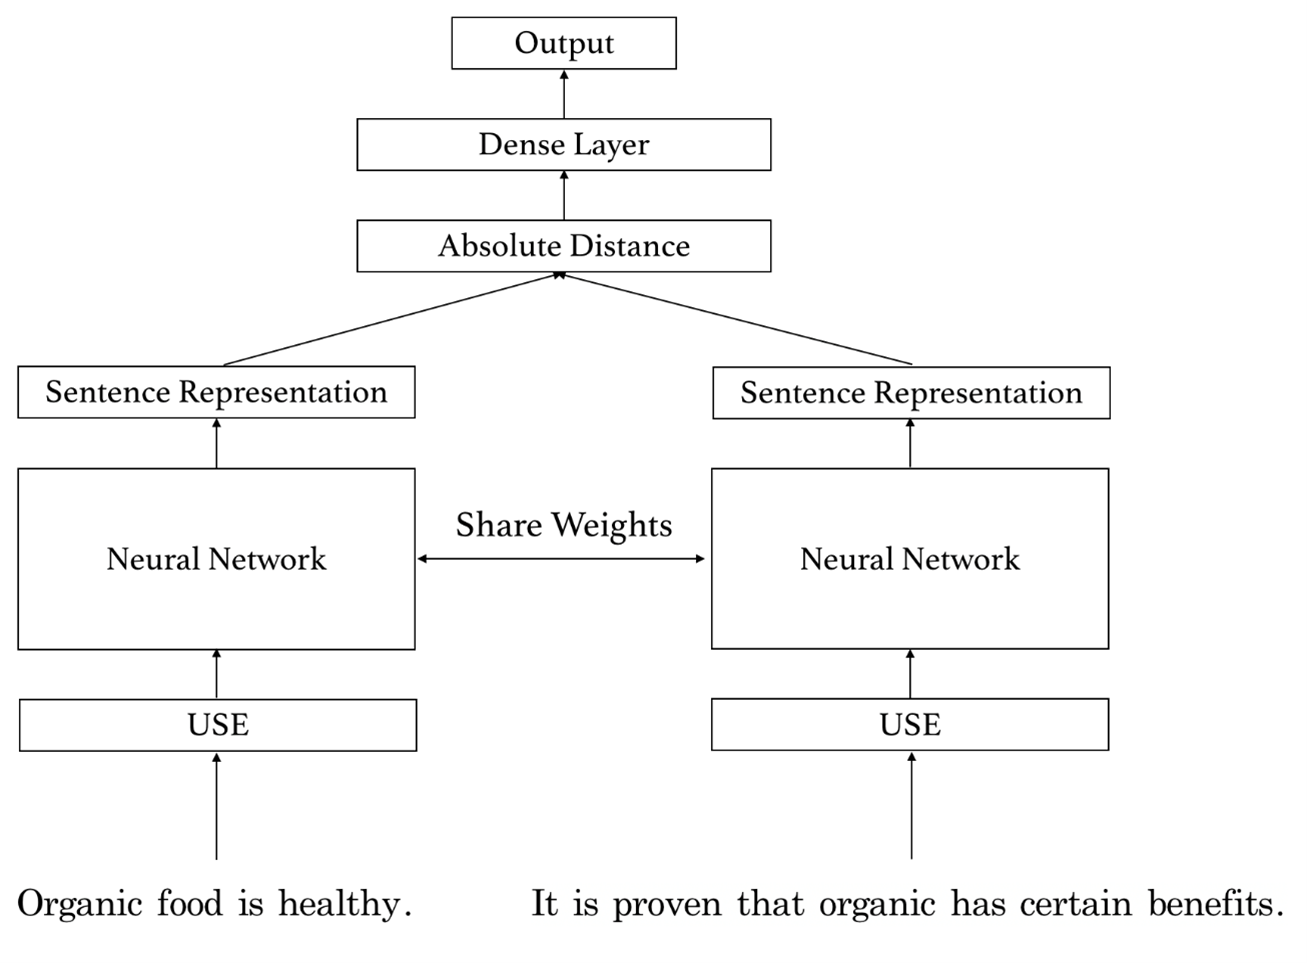
\includegraphics[scale=0.47]{it18149654_siamese.png}}}
\caption{Siamese Network Architecture}
\end{figure}

Each data set was analyzed and cleaned for records with any null values or duplicates. Basic text preprocessing such as removing HTML tags, invalid special characters, punctuations, and contractions was performed using regular expressions for text data in the data sets. NLP preprocessing techniques such as stop-words removal, lemmatization, and tokenization were performed using the NLTK library. Tokenizer and pad\_sequences from Keras library were used to transform textual data into a sequence of integers before feeding them to the learning algorithm. Deep learning models with Siamese neural network architecture as shown in Fig. 6, were trained. Models were trained with different preprocessing techniques (with and without lemmatization of textual data) and varying the hyper-parameter values such as the epochs count to determine the optimum model.

For spelling and grammar checking of the submitted student answer, the GrammarBot library was used which responds with violated grammatical rule type and suggested corrections for each identified grammatical and spelling mistake. TextBlob library was used to measure the subjectivity of the submitted answer using TextBlob Sentiment which consists of polarity and subjectivity scores for a provided textual input. Fig. 7 shows a high-level architecture diagram of the semantic similarity evaluation component.

\begin{figure}[htbp]
\centerline{\frame{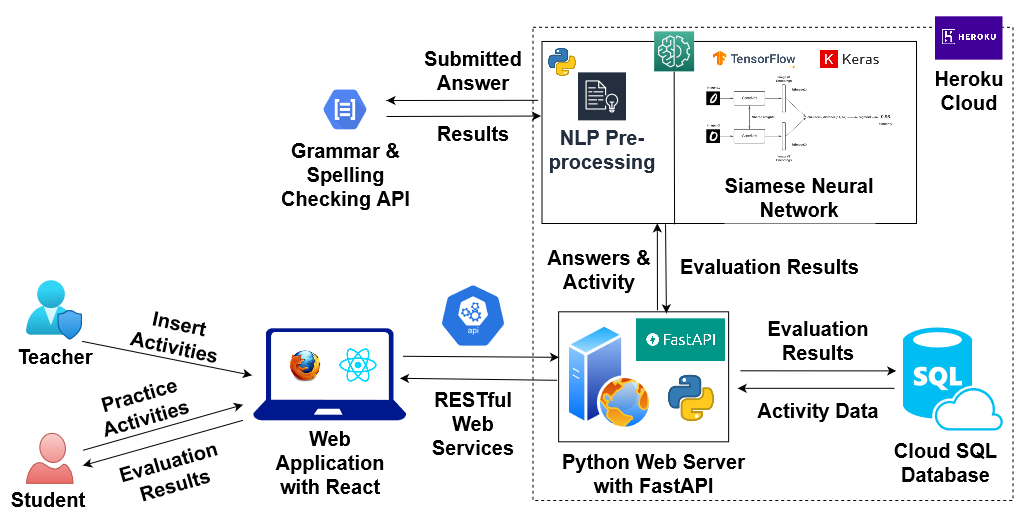
\includegraphics[scale=0.32]{it18149654_sod.png}}}
\caption{System Diagram for Semantic Similarity Evaluation Component}
\end{figure}

The deep learning models for written activity evaluation were evaluated using different evaluation metrics. A qualified and experienced human evaluator in English exams is hired to validate the accuracy of both the speaking and writing activities evaluation predictions by the learning algorithms. The effect of the recommendation system implemented using the Q-Learning algorithm is evaluated by comparing random contents suggestion as opposed to recommended content suggestions to users and getting their feedback.

\section{Results and Discussion}

Each component of the system uses different evaluation processes to measure the accuracy since achieving highly accurate outputs was a major priority when developing the system. The system provides unbiased and accurate results and recommendations while saving time and resources by automating the manual work.

\subsection{Automated Pronunciation Error Detection and Evaluation}

This component used vowel sounds to detect pronunciation errors of the user. The biggest challenge was to identify vowels within the words and measure formant frequency within the vowel duration. The developed algorithm was able to detect vowel occurring pleases automatically and measure formant frequency within the vowel duration. Accuracy was measured by comparing measured values from the Praat tool manually. The result of the manual measuring process with the Praat tool and the result measured with an automated algorithm is shown in Table 1.

\begin{table}[htbp]
\centering
\scriptsize
Table 1. Praat Tool vs. English Buddy
\linebreak
\linebreak
\centerline{\frame{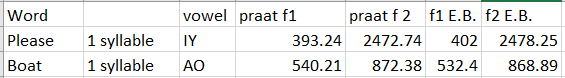
\includegraphics[scale=0.59]{IT18151220_results.png}}}
\end{table}

The intelligent virtual tutor takes the role of a private tutor for the student. Such a tutor would have the means of providing corrective audio-visual feedback. It includes illustrating the differences between a speaker’s pronunciation and a reference speaker, in a manner that helps non-native speakers to figure out how to reduce their accent.

\subsection{Personalized Learning \& Real-Time Sentiment Analysis}
 
This component was evaluated with particular student activities and provided suggestions according to the results, current state, and ratings. The system consists of real-time sentiment analysis which automatically rates the course contents according to the user feedback.

\begin{center}
\scriptsize
Table 2. Sentiment Analysis Model Evaluation
\linebreak
\linebreak
\scriptsize
\begin{tabular}{ | m{13em} | m{3em} | }
\hline
\raggedright
Metric & Value \\
\hline
\raggedright
Average Micro Accuracy & 0.916 \\
\hline
\raggedright
Average Macro Accuracy & 0.813 \\
\hline
\end{tabular}
\linebreak
\end{center}

As shown in Table 2, the achieved average Micro Accuracy and Macro Accuracy for the Sentiment analysis model were 0.916 and 0.813 respectively. The average Log-Loss function and the average Log-Loss Reduction of the model were 0.433 respectively. Further, Fig. 8 shows the output of the Q-matrix.

\begin{figure}[htbp]
\small
\centerline{\frame{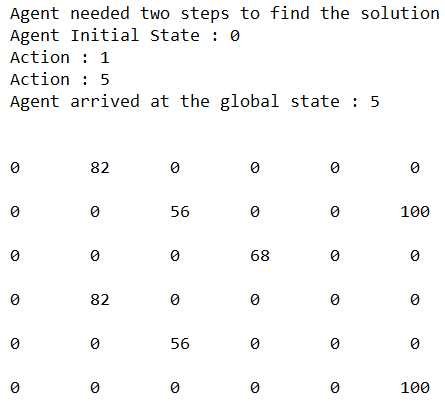
\includegraphics[scale=0.34]{it18153682_q_matrix.png}}}
\caption{Q-Matrix Output}
\end{figure}

Furthermore, the User Acceptance Testing (UAT), which was conducted with 3 end-users, proved that the personalized recommendations are reliable.

\subsection{Automated Essay Evaluation}

The dropout layer of the LSTM model had been used to improve the performance of the model by preventing over-fitting. The Cohens Kappa value was calculated with quadratic weights 5 times using KFold cross-validation. The model achieved 0.93 average Cohen’s Kappa which is significantly higher and reveals there is a near-perfect agreement. The average Weighted Kappa value for a solution with a machine learning approach was just 0.73 [23]. Therefore, the results indicate that the deep learning-based approach performs significantly better than machine learning approaches.

\subsection{Semantic Textual Similarity Evaluation}

Several deep learning models with Siamese network architecture were trained to measure the semantic textual similarity using several data sets with different preprocessing techniques. A simple comparison of the model evaluation revealed that the QQP data set with performing lemmatization to textual data produced the best results when trained with 5 epochs.

\begin{center}
\scriptsize
Table 3. Evaluation Metrics for Siamese Network Models
\linebreak
\linebreak
\scriptsize
\begin{tabular}{ | m{7em} | m{7em} | m{7em} | }
\hline
\raggedright
Eval. Metric & With Lemma. & Without Lemma. \\
\hline
\raggedright
Train Accuracy & 0.8477 & 0.8452 \\
\hline
\raggedright
Validation Acc. & 0.8087 & 0.8071 \\
\hline
\raggedright
MAE & 0.2475 & 0.2421 \\
\hline
\raggedright
MSE & 0.1338 & 0.1352 \\
\hline
\raggedright
RMSE & 0.3658 & 0.3677 \\
\hline
\end{tabular}
\linebreak
\end{center}

Table 3 shows the evaluation results for various Siamese network models trained with the QQP data set. The optimum model obtained an accuracy of 0.8087.

\section{Limitations and Future Work}

In the future, the implemented deep learning algorithms can be enhanced to improve their accuracy and decrease over-fitting-related issues by expanding training data by combining multiple similar data sets. Hyper-parameters like epochs count can be fine-tuned and text pre-processing techniques can be varied. Novel deep learning model architectures such as Transformer and Graph neural networks can be tried out in written activity evaluation functionalities. Evaluating handwritten answers using Handwritten Text Recognition can be implemented. The system can be extended to other languages.

\section{Conclusion}

This research focuses on developing a system to enhance the learning experience and improve proficiency in the English language among non-native speakers. The system provides an all-in-one solution including a personalized learning environment, automated pronunciation error detection, automated essay evaluation, automated descriptive answer evaluation based on semantic similarity, and a real-time course content rating system. The system is implemented using Audio Signal Processing, Reinforcement Learning, Deep Learning, and NLP. Accuracy values for the LSTM, Sentiment Analysis, and Siamese network models used in this research are 0.93, 0.92, and 0.81 respectively. Further, the results of UAT demonstrated that the personalized recommendations and pronunciation error detection processes are accurate. This system was able to provide better results and overcome the shortcomings of the existing solutions that utilize traditional methodologies.

\begin{thebibliography}{00}

\raggedright

\bibitem{b1} ``The Importance of the English Language: 10 Reasons to Learn English'', BSC (EN), 2021. [Online]. Available: www.british-study.com/en/importance-of-english-language.
\bibitem{b2} ``4 reasons why learning English is essential'', Etsglobal.org, 2020. [Online]. Available: www.etsglobal.org/pl/en/blog/news/importance-of-learning-english.
\bibitem{b3} J. Weingarten, ``The Complete Guide to English-Language Certificates - MastersPortal.com'', Mastersportal.com, 2021. [Online]. Available: www.mastersportal.com/articles/345/the-complete-guide-to-english-language-certificates.ht.
\bibitem{b4} ``Literacy rate, adult total (percentage of people aged 15 and above) - Sri Lanka | Data'', Data.worldbank.org, 2021. [Online]. Available: data.worldbank.org/indicator/SE.ADT.LITR.ZS?ml.
\bibitem{b5} A. Abayasekara, ``Building a More English-Literate Sri Lanka: The Need to Combat Inequities'', Ips.lk, 2018. [Online]. Available: www.ips.lk/talkingeconomics/2018/04/23/building-a-more-english-literate-sri-lanka-the-need-to-combat-inequities.
\bibitem{b6} B. S. J. Kapoor, S. M. Nagpure, S. S. Kolhatkar, P. G. Chanore, M. M. Vishwakarma and R. B. Kokate, ``An Analysis of Automated Answer Evaluation Systems based on Machine Learning,'' 2020 International Conference on Inventive Computation Technologies (ICICT), Coimbatore, India, 2020, pp. 439-443, doi: 10.1109/ICICT48043.2020.9112429.
\bibitem{b7} C. J. C. H. Watkins and P. Dayan, ``Q-learning,'' Machine Learning, vol. 8, pp. 279-292. 1992.
\bibitem{b8} H. Mahfoodh and H. AlAtawi, ``Sustaining Higher Education through eLearning in Post Covid-19,'' 2020 Sixth International Conference on e-Learning (econf), 2020, pp. 361-365, doi: 10.1109/econf51404.2020.9385477.
\bibitem{b9} Du Li, Lin Zhuying and Yin Bing, ``The application of AI technology in Intelligent Tutoring System,'' 2010 2nd International Conference on Education Technology and Computer, 2010, pp. V1-490-V1-493, doi: 10.1109/ICETC.2010.5529201.
\bibitem{b10} Y. Wang, Y. Sun, and Y. Chen, ``Design and Research of Intelligent Tutor System Based on Natural Language Processing,'' 2019 IEEE International Conference on Computer Science and Educational Informatization (CSEI), 2019, pp. 33-36, doi: 10.1109/CSEI47661.2019.8939031.
\bibitem{b11} Yoon Kim, Horacio Franco, and Leonardo Neumeyer. ``Automatic pronunciation scoring of specific phone segments for language instruction,'' Eurospeech, Rhodes, Greece, 1997.
\bibitem{b12} B. Mak, M. Siu, M. Ng, Yik-Cheung Tam, Yu-Chung Chan, Kin-Wah Chan, Ka-Yee Leung, S. Ho, Fong-Ho Chong, J. Wong, and J. Lo. ``PLASER: Pronunciation learning via automatic speech recognition.,'' Proc. HLT-NAACL 2003 Workshop on Building Educational Applications Using Natural Language Processing, pages 23–29, 2003.
\bibitem{b13} R. Delmonte. ``Exploring Speech Technologies for Language Learning'', June 2011. [Online]. Available: www.intechopen.com/books/speech-and-language-technologies.
\bibitem{b14} J. Bernstein, J. Cheng, M. Suzuki. ``Fluency changes with general progress in L2 proficiency,'' Interspeech 2011, Florence, Italy, 2011.
\bibitem{b15} Pieter Mueller, Febe de Wet, Christa van der Walt, and Thomas Niesler. ``Automatically assessing the oral proficiency of proficient L2 speakers,'' SLaTE 2009, Birmingham, England, 2009.
\bibitem{b16} S. Schiaffino, P. Garcia, and A. Amandi, ``eTeacher: Providing personalized assistance to e-learning students,'' Compute. Educ., vol. 51, no. 4, pp. 1744–1754, Dec. 2008, doi: 10.1016/j.compedu.2008.05.008.
\bibitem{b17} M. S. Halawa, E. M. R. Hamed, and M. E. Shehab, ``Personalized E-learning recommendation model based on the psychological type \& learning style models,'' 2015 IEEE 7th Int. Conf. Intell. Comput. Inf. Syst. ICICIS 2015, pp. 578–584, 2016, doi: 10.1109/IntelCIS.2015.7397281.
\bibitem{b18} P. Yang, Y. Wang, J. P. Li, and B. Kong, ``Study on personality learning in E-learning,'' 2009 Int. Conf. E-learning, E-Business, Enterp. Inf. Syst. E-Government, EEEE 2009, pp. 126–128, 2009, doi: 10.1109/EEEE.2009.39.
\bibitem{b19} M. Prasad, G. Himaja, C. Abhigna, K. Saroja and K. Venkatesh, ``Automated Essay Grading System Using Deep Learning,'' Dept. Of Computer Science and Engineering, Dhanekula Institute of Engineering and Technology, Andhra Pradesh, India, 2020.
\bibitem{b20} A. Shehab, M. Elhoseny and A. E. Hassanien, ``A hybrid scheme for Automated Essay Grading based on LVQ and NLP techniques,'' 2016 12th International Computer Engineering Conference (ICENCO), Cairo, Egypt, 2016, pp. 65-70, doi: 10.1109/ICENCO.2016.7856447.
\bibitem{b21} J. Bromley et al., ``Signature Verification using a Siamese Time Delay Neural Network,'' International Journal of Pattern Recognition and Artificial Intelligence, vol. 07, no. 04. World Scientific Pub Co Pte Lt, pp. 669–688, Aug. 1993. doi: 10.1142/s0218001493000339.
\bibitem{b22} C. Jin and B. He, ``Utilizing Latent Semantic Word Representations for Automated Essay Scoring,'' 2015 IEEE 15th Intl Conf on Scalable Computing and Communications \& Its Associated Workshops (UIC-ATC-ScalCom), Beijing, China, 2015, pp. 1101-1108, doi: 10.1109/UIC-ATC-ScalCom-CBDCom-IoP.2015.202.
\bibitem{b23} M. Mahana, M. Johns, and A. Apte, ``Automated Essay Grading Using Machine Learning,'' CS229 Machine Learning - Autumn 2012 Stanford University, 2012, p. citeseerx.ist.psu.edu.
\bibitem{b24} D. Verma and S. N. Muralikrishna, ``Semantic similarity between short paragraphs using Deep Learning,'' 2020 IEEE International Conference on Electronics, Computing and Communication Technologies (CONECCT), Bangalore, India, 2020, pp. 1-5, doi: 10.1109/CONECCT50063.2020.9198445.
\bibitem{b25} S. S. Senevirathne et al., ``Smart Personal Intelligent Assistant for Candidates of IELTS Exams,'' 2020 2nd International Conference on Advancements in Computing (ICAC), Malabe, Sri Lanka, 2020, pp. 446-451, doi: 10.1109/ICAC51239.2020.9357150.
\bibitem{b26} M. Indu and K. V. Kavitha, ``Review on text summarization evaluation methods,'' 2016 International Conference on Research Advances in Integrated Navigation Systems (RAINS), Bangalore, India, 2016, pp. 1-4, doi: 10.1109/RAINS.2016.7764406.
\bibitem{b27} M. M. Rahman and F. H. Siddiqui, ``NLP-based Automatic Answer Script Evaluation,'' DUET J., vol. 35, no. 1, 2018.
\bibitem{b28} R. Goswami, S. Karmakar, A. Bisai and A. R. Pal, ``A knowledge-based approach for long answer evaluation,'' 2017 2nd IEEE International Conference on Recent Trends in Electronics, Information \& Communication Technology (RTEICT), Bangalore, India, 2017, pp. 773-777, doi: 10.1109/RTEICT.2017.8256702.

\end{thebibliography}

\end{document}
